\documentclass{article}
\usepackage{amsmath}
\usepackage{amsfonts}
\usepackage{amssymb}
\usepackage{graphicx}
\usepackage{hyperref}
\usepackage[backend=biber,style=numeric]{biblatex}
\addbibresource{notes-01-mlp/reference.bib}
\hypersetup{
    colorlinks=true,   
    linkcolor=black,  
    urlcolor=blue      
}
\usepackage[T2A]{fontenc} 
\usepackage[utf8]{inputenc}
\usepackage[russian, english]{babel} 
\usepackage{pgfplots} 
\pgfplotsset{compat=1.8} 
\setcounter{secnumdepth}{0}
\graphicspath{ {notes-01-mlp} }
\title{Deep Learning - Lecture 1}
\author{Kalinin Nikita}
\date{}

\begin{document}

\maketitle
\tableofcontents
\newpage

\section{Core Concepts}
\begin{itemize}
    \item \textbf{Backpropagation}: A key algorithm for training neural networks by propagating the error backwards through the network to adjust the weights.
    \item \textbf{Fully-connected Networks}: Each neuron is connected to every neuron in the previous layer, making them suitable for tasks like classification.
\end{itemize}

\section{Mathematical Notation and Definitions}

Let the input features be represented as:
\[
\{(x_i, y_i)\}_{i=1}^{l}
\]
where \( x_i \in \mathbb{R}^d \) is an input vector, and \( y_i \) is the corresponding target value. Here:
\begin{itemize}
    \item \( x \in \mathbb{R}^d \): Input vector with \( d \) dimensions.
    \item \( \mathbf{w} \in \mathcal{W} \): Weight vector of the neural network.
\end{itemize}

The network's output for an input \( x \) can be written as:
\[
a(x) = w_1 x_1 + \dots + w_d x_d = f(x, \mathbf{w})
\]

Given a training set, the goal is to minimize the loss function \( L(\hat{y}, y) \), where:
\[
Q(\mathbf{w}) = \frac{1}{l} \sum_{i=1}^{l} L\left( f(x_i, \mathbf{w}), y_i \right)
\]
This represents the average loss across all samples in the training set. The aim is to find the optimal weights \( \mathbf{w} \) that minimize \( Q(\mathbf{w}) \).

\section{Alternatives to Backpropagation}

Historically, other methods have been explored as alternatives to backpropagation:

\subsubsection{Historic Approaches}
\begin{itemize}
    \item \textbf{Evolutionary Algorithms (1950s)}\cite{evolutionary_algorithms}: Optimization methods inspired by natural selection, often computationally expensive for large networks.
    \item \textbf{Reservoir Computing (2000)}\cite{dong2020reservoir}: Uses fixed random weights in a large recurrent neural network (RNN), making it useful for certain tasks, especially where the input is sequential.
\end{itemize}

\subsubsection{Modern Approaches}
\begin{itemize}
    \item \textbf{Direct Feedback Alignment (2016)}\cite{nokland2016dfa}: A variant of backpropagation where the feedback path does not use the exact gradients but rather a fixed random path.
    \item \textbf{Forward-Forward Algorithm (2022)}\cite{hinton2022forward}: A recent approach that aims to replace backpropagation by only using forward passes, potentially reducing the complexity and computational cost of training.
\end{itemize}

\section{Gradient Calculation for Neural Networks}
In neural networks, the output \( y \) is often a function of intermediate layers:
\[
y = f(g(x))
\]
The gradient can be calculated as:
\[
\frac{dy}{dx} = \frac{dy}{df} \cdot \frac{dg}{dx}
\]
where \( g(x) \) represents an intermediate transformation of the input \( x \), and \( \frac{dy}{df} \) is calculated based on the loss with respect to the output layer.


\section{Backpropagation}

1. For a composition of functions, let:
   \[
   y = f(g(x))
   \]
   Then the derivative \( \frac{dy}{dx} \) is given by the chain rule:
   \[
   \frac{dy}{dx} = \frac{df}{dg} \cdot \frac{dg}{dx}
   \]

2. More generally, if \( y = f(g_1(x), g_2(x), \dots, g_n(x)) \), then:
   \[
   \frac{dy}{dx} = \sum_{i=1}^{n} D_i f \cdot \frac{dg_i}{dx}
   \]
   where:
   \[
   D_i f = \frac{\partial f}{\partial z_i}
   \]
   and \( f(z_1, \dots, z_n) \) represents a function of multiple variables \( z_i \).

\subsection{Symbolic vs Numeric Differentiation}
\begin{itemize}
\item \textbf{Symbolic Differentiation}: For expressions like \( x^2 \), differentiation yields \( 2x \) for all \( x \).

\item \textbf{Numeric Differentiation}: For expressions like \( x^2 \) with a specific value \( x := 3 \), differentiation yields a concrete result, e.g., \( 6 \).
\end{itemize}

\section{Computational Graph}

Consider the function:
\[
f = x_1^2 (x_2 x_3 - 2 x_1^2) = x_1^2 x_2 x_3 - 2 x_1^4
\]

Calculating partial derivatives with respect to each \( x_i \):

\begin{align*}
\frac{\partial f}{\partial x_1} &= 2 x_1 x_2 x_3 - 8 x_1^3 = 4 \quad \text{(when \( x = (1, 2, 3) \))}, \\
\frac{\partial f}{\partial x_2} &= x_1^2 x_3 = 3, \\
\frac{\partial f}{\partial x_3} &= x_1^2 x_2 = 2.
\end{align*}

Given \( x = (1, 2, 3) \), we can calculate \( y \) as:
\[
y = x_1^2 (x_2 x_3 - 2 x_1^2)
\]

Substituting values:
\[
y = 1^2 (2 \cdot 3 - 2 \cdot 1^2) = 1 \cdot (6 - 2) = 4
\]


\section{Computational Graph Example}

For the function:
\[
y = z_1 z_4, \quad \text{where} \quad z_1 = x_1^2, \quad z_2 = x_2 x_3, \quad z_3 = 2 z_1, \quad z_4 = z_2 - z_3
\]

\subsection{Forward Pass}
\begin{align*}
z_1 &= x_1^2, \\
z_2 &= x_2 x_3, \\
z_3 &= 2 z_1, \\
z_4 &= z_2 - z_3, \\
y &= z_1 z_4.
\end{align*}

\subsection{Backward Pass}
Using the chain rule for each variable:

\[
\frac{dy}{dy} = 1
\]

\begin{align*}
\frac{dy}{dz_4} &= \frac{dy}{dy} \cdot z_1 = 1 \cdot z_1 = 1, \\
\frac{dy}{dz_3} &= \frac{dy}{dz_4} \cdot \frac{dz_4}{dz_3} = 1 \cdot (-1) = -1, \\
\frac{dy}{dz_2} &= z_4 \cdot 1 + \frac{dy}{dz_3} \cdot \frac{dz_3}{dz_1} = 4 + (-1) \cdot 2 = 2.
\end{align*}

Finally, for \( x \):
\[
\frac{dy}{dx_1} = \frac{dy}{dz_1} \cdot \frac{dz_1}{dx_1}, \quad \frac{dy}{dx_2} = \frac{dy}{dz_2} \cdot \frac{dz_2}{dx_2}, \quad \frac{dy}{dx_3} = \frac{dy}{dz_2} \cdot \frac{dz_2}{dx_3}.
\]


\section{Neural Network Layers}

Let \( x \in \mathbb{R}^d \) and \( w \in \mathbb{R}^d \) be the input and weight vectors:
\[
a(x) = \langle w, x \rangle = w^T x.
\]

Consider a multi-layer network:
\[
z_1 = W_1 x + b_1, \quad z_2 = W_2 z_1 + b_2, \dots, \quad z_n = W_n z_{n-1} + b_n
\]
where \( W_i \in \mathbb{R}^{d_i \times d_{i-1}} \) and \( b_i \in \mathbb{R}^{d_i} \).

The output layer can be represented as:
\[
z_n = W_n \dots W_2 W_1 x + b
\]
with weights \( W \in \mathbb{R}^{d_n \times d} \).

Let \( \sigma(\cdot) \) be the activation function:
\[
z_i = \sigma(W_i z_{i-1} + b_i).
\]

\section{Neural Network Architectures}

A \textbf{dense layer} (also known as a \textbf{fully-connected layer}) computes a latent representation \( z_i \) as a combination of inputs from the previous layer.

\[
z_i = \left( z_i^{(1)}, \dots, z_i^{(d_i)} \right)
\]

\begin{figure}[h]
    \centering
    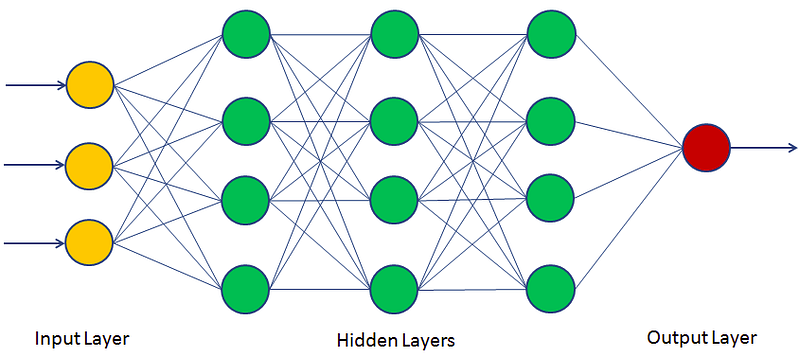
\includegraphics[width=0.4\textwidth]{MLP.png}
    \caption{Multi-Layer Perceptron}
    \label{fig:rotated_image}
\end{figure}

Each neuron in the layer is connected to all neurons in the previous layer.


\textbf{MLP} (Multi-Layer Perceptron): A type of fully-connected network with one or more hidden layers. \textbf{FCN} (Fully Connected Network): Another term for a neural network with fully-connected layers.


\subsection{Layer Calculations}
In a typical layer, we have:
\[
u_i = W_i z_i + b_i, \quad z_{i+1} = \sigma(u_i)
\]
The gradient of the error \( E \) with respect to \( z_i \) can be computed as:
\[
\frac{dE}{dz_i} = \frac{dE}{dz_{i+1}} \cdot \sigma'(u_i) \frac{du_i}{dz_i}
\]
where \( \sigma'(u_i) \) can become very small, contributing to the vanishing gradient issue.

\section{Activation Functions and Vanishing Gradients}

One common issue in training deep neural networks is the \textbf{vanishing gradient problem}. It occurs when gradients diminish as they propagate back through the layers, which can significantly slow down or even halt the learning process in earlier layers.

\subsection{1. Sigmoid Activation Function}
The sigmoid function is defined as:
\[
\sigma(x) = \frac{1}{1 + e^{-x}}
\]
Its derivative, important for gradient calculations in backpropagation, is:
\[
\sigma'(x) = \sigma(x) (1 - \sigma(x)) = \frac{e^{-x}}{(1 + e^{-x})^2}
\]

\begin{figure}[h]
    \centering
    \begin{tikzpicture}
        \begin{axis}[
            axis lines=middle,
            xlabel={$x$},
            ylabel={$f(x), f'(x)$},
            samples=100,
            domain=-10:10,
            width=10cm,
            height=6cm,
            ymin=-0.1, ymax=1.1,
            xtick={-10,-5,0,5,10},
            ytick={0,0.5,1},
            legend style={at={(0.5,-0.2)}, anchor=north, legend columns=-1},
            legend entries={$\sigma(x)$, $\sigma'(x)$},
        ]
            \addplot[smooth, thick, blue] {1 / (1 + exp(-x))};
            
            \addplot[smooth, thick, red, dashed] {
                (1 / (1 + exp(-x))) * (1 - (1 / (1 + exp(-x))))
            };
        \end{axis}
    \end{tikzpicture}
    \caption{Sigmoid activation function and its derivative}
    \label{fig:sigmoid_derivative}
\end{figure}
\newpage

\subsection{2. ReLU (Rectified Linear Unit)}
The ReLU function is defined as:
\[
\text{ReLU}(x) = \max(0, x)
\]
The derivative of ReLU, which is 1 for positive inputs and 0 for negative inputs, helps to mitigate the vanishing gradient problem by allowing gradients to propagate effectively for positive activations.

\[
\text{ReLU}'(x) = 
\begin{cases} 
1, & x > 0 \\ 
0, & x \leq 0 
\end{cases}
\]

\begin{figure}[h]
    \centering
    \begin{tikzpicture}
        \begin{axis}[
            axis lines=middle,
            xlabel={$x$},
            ylabel={$f(x)$},
            ymin=-1, ymax=3,
            xmin=-3, xmax=3,
            samples=100,
            domain=-3:3,
            width=8cm, height=6cm,
            grid=both,
            xtick={-2, -1, 0, 1, 2},
            ytick={0, 1, 2},
            legend style={at={(1,1)}, anchor=north east}
        ]
            \addplot[red, thick] {max(0, x)} node[pos=0.8, above] {ReLU$(x)$};
        \addlegendentry{ReLU$(x)$};
        
        \addplot[green, thick, dashed] {x >= 0 ? 1 : 0} node[pos=0.3, below];
        \addlegendentry{ReLU$'(x)$};
        \end{axis}
\end{tikzpicture}
\caption{ReLU activation function}
\label{fig:relu}
\end{figure}

\subsection{3. Leaky ReLU}
Leaky ReLU introduces a small slope \( \alpha \) for negative values, defined as:
\[
\text{Leaky ReLU}(x) = \max(\alpha x, x)
\]
This small gradient for negative inputs (controlled by \( \alpha \)) ensures that neurons do not become inactive during training.

\begin{figure}[h]
    \centering
\begin{tikzpicture}
    \begin{axis}[
        axis lines=middle,
        xlabel={$x$},
        ylabel={$f(x)$},
        ymin=-1, ymax=3,
        xmin=-3, xmax=3,
        samples=100,
        domain=-3:3,
        width=8cm, height=6cm,
        grid=both,
        xtick={-2, -1, 0, 1, 2},
        ytick={0, 1, 2},
        legend style={at={(1,1)}, anchor=north east}
    ]
        \addplot[red, thick] {x >= 0 ? x : 0.1 * x} node[pos=0.8, above] {Leaky ReLU$(x)$};
        \addlegendentry{Leaky ReLU$(x)$};

        \addplot[green, thick, dashed] {x >= 0 ? 1 : 0.1} node[pos=0.3, below];
        \addlegendentry{Leaky ReLU$'(x)$};
        % Add alpha annotation for the slope
        \draw[<->, thick, blue] (axis cs:-2, -0.2) -- (axis cs:-2, -0.1) node[midway, left] {$\alpha$};
        \end{axis}
\end{tikzpicture}
\caption{Leaky ReLU activation function}
\label{fig:leaky_relu}
\end{figure}

\printbibliography

\end{document}


